\documentclass[border=6mm,tikz]{standalone}
\begin{document}
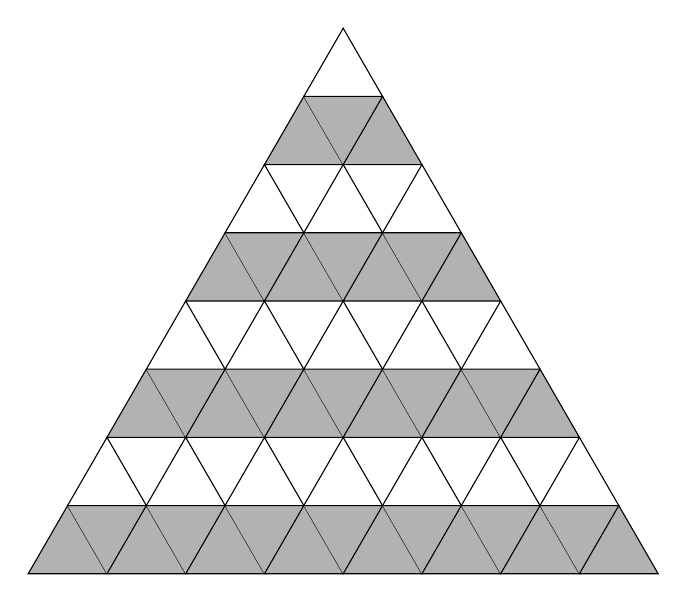
\begin{tikzpicture}
	\foreach \i[evaluate = \i as \k using int(8-\i-1)] in {0,...,7}{
         \foreach \j in {0,...,\k}{
            \ifodd \i
                \draw[shift={(60:\i)},shift={(\j,0)}] (0,0)--(0:1)--(60:1)--cycle;
            \else{
                \draw[shift={(60:\i)},shift={(\j,0)},fill=gray!60] (0,0)--(0:1) -- (60:1) -- cycle;
                \ifnum \j<\k\relax
                    \fill[shift={(60:\i)},shift={(\j,0)},gray!60] (60:1) -- ++(1,0) -- ++(-120:1);
                \else\fi
            }
            \fi
         }
    }
\end{tikzpicture}
\end{document}